\chapter{矩阵}

\index{matrix}

\key{矩阵}是一种数学概念，对应程序中的二维数组。例如，
\[
A = 
 \begin{bmatrix}
  6 & 13 & 7 & 4 \\
  7 & 0 & 8 & 2 \\
  9 & 5 & 4 & 18 \\
 \end{bmatrix}
\]
是一个 $3 \times 4$ 矩阵，即它有 3 行 4 列。记号 $[i,j]$ 表示矩阵中第 $i$ 行、第 $j$ 列的元素。例如，在上述矩阵中，$A[2,3]=8$，$A[3,1]=9$。

\index{vector}

矩阵的一种特殊情形是\key{向量}，即大小为 $n \times 1$ 的一维矩阵。例如，
\[
V =
\begin{bmatrix}
4 \\
7 \\
5 \\
\end{bmatrix}
\]
是一个包含三个元素的向量。

\index{transpose}

矩阵 $A$ 的\key{转置} $A^T$ 通过交换 $A$ 的行与列得到，即 $A^T[i,j]=A[j,i]$：
\[
A^T = 
 \begin{bmatrix}
  6 & 7 & 9 \\
  13 & 0 & 5 \\
  7 & 8 & 4 \\
  4 & 2 & 18 \\
 \end{bmatrix}
\]

\index{square matrix}

如果矩阵的行数和列数相同，就称它为\key{方阵}。例如，下面的矩阵是方阵：

\[
S = 
 \begin{bmatrix}
  3 & 12 & 4  \\
  5 & 9 & 15  \\
  0 & 2 & 4 \\
 \end{bmatrix}
\]

\section{运算}

当矩阵 $A$、$B$ 大小相同时，可以定义它们的和 $A+B$。结果矩阵中的每个元素等于 $A$、$B$ 对应位置元素之和。

例如，
\[
 \begin{bmatrix}
  6 & 1 & 4 \\
  3 & 9 & 2 \\
 \end{bmatrix}
+
 \begin{bmatrix}
  4 & 9 & 3 \\
  8 & 1 & 3 \\
 \end{bmatrix}
=
 \begin{bmatrix}
  6+4 & 1+9 & 4+3 \\
  3+8 & 9+1 & 2+3 \\
 \end{bmatrix}
=
 \begin{bmatrix}
  10 & 10 & 7 \\
  11 & 10 & 5 \\
 \end{bmatrix}.
\]

矩阵 $A$ 乘以数值 $x$，表示把 $A$ 的每个元素都乘以 $x$。例如，
\[
 2 \cdot \begin{bmatrix}
  6 & 1 & 4 \\
  3 & 9 & 2 \\
 \end{bmatrix}
=
 \begin{bmatrix}
  2 \cdot 6 & 2\cdot1 & 2\cdot4 \\
  2\cdot3 & 2\cdot9 & 2\cdot2 \\
 \end{bmatrix}
=
 \begin{bmatrix}
  12 & 2 & 8 \\
  6 & 18 & 4 \\
 \end{bmatrix}.
\]

\subsubsection{矩阵乘法}

\index{matrix multiplication}

当 $A$ 的大小为 $a \times n$、$B$ 的大小为 $n \times b$ 时，即 $A$ 的列数等于 $B$ 的行数时，可以定义矩阵乘积 $AB$。结果是一个 $a \times b$ 矩阵，其元素按公式
\[
AB[i,j] = \sum_{k=1}^n A[i,k] \cdot B[k,j].
\]

计算。也就是说，$AB$ 的每个元素都是 $A$ 的一行与 $B$ 的一列对应元素乘积之和，如下图所示：

\begin{center}
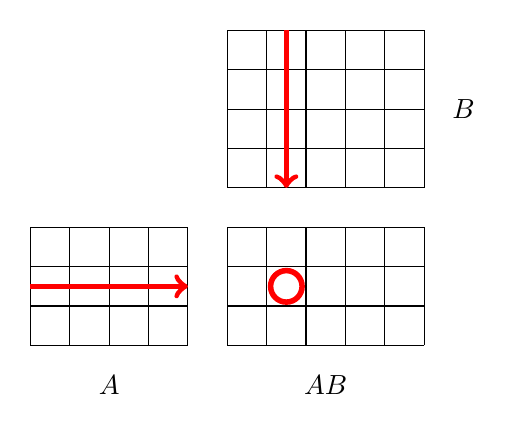
\begin{tikzpicture}[scale=0.5]
\draw (0,0) grid (4,3);
\draw (5,0) grid (10,3);
\draw (5,4) grid (10,8);

\node at (2,-1) {$A$};
\node at (7.5,-1) {$AB$};
\node at (11,6) {$B$};

\draw[thick,->,red,line width=2pt] (0,1.5) -- (4,1.5);
\draw[thick,->,red,line width=2pt] (6.5,8) -- (6.5,4);
\draw[thick,red,line width=2pt] (6.5,1.5) circle (0.4);
\end{tikzpicture}
\end{center}

例如，

\[
 \begin{bmatrix}
  1 & 4 \\
  3 & 9 \\
  8 & 6 \\
 \end{bmatrix}
\cdot
 \begin{bmatrix}
  1 & 6 \\
  2 & 9 \\
 \end{bmatrix}
=
 \begin{bmatrix}
  1 \cdot 1 + 4 \cdot 2 & 1 \cdot 6 + 4 \cdot 9 \\
  3 \cdot 1 + 9 \cdot 2 & 3 \cdot 6 + 9 \cdot 9 \\
  8 \cdot 1 + 6 \cdot 2 & 8 \cdot 6 + 6 \cdot 9 \\
 \end{bmatrix}
=
 \begin{bmatrix}
  9 & 42 \\
  21 & 99 \\
  20 & 102 \\
 \end{bmatrix}.
\]

矩阵乘法满足结合律，即 $A(BC)=(AB)C$；但通常不满足交换律，即一般有 $AB \ne BA$。

\index{identity matrix}

\key{单位矩阵}是主对角线元素全为 1、其他元素全为 0 的方阵。例如，下面是 $3 \times 3$ 单位矩阵：
\[
 I = \begin{bmatrix}
  1 & 0 & 0 \\
  0 & 1 & 0 \\
  0 & 0 & 1 \\
 \end{bmatrix}
\]

\begin{samepage}
矩阵乘以单位矩阵后保持不变。例如，
\[
 \begin{bmatrix}
  1 & 0 & 0 \\
  0 & 1 & 0 \\
  0 & 0 & 1 \\
 \end{bmatrix}
\cdot
 \begin{bmatrix}
  1 & 4 \\
  3 & 9 \\
  8 & 6 \\
 \end{bmatrix}
=
 \begin{bmatrix}
  1 & 4 \\
  3 & 9 \\
  8 & 6 \\
 \end{bmatrix} \hspace{10pt} \textrm{且} \hspace{10pt}
 \begin{bmatrix}
  1 & 4 \\
  3 & 9 \\
  8 & 6 \\
 \end{bmatrix}
\cdot
 \begin{bmatrix}
  1 & 0 \\
  0 & 1 \\
 \end{bmatrix}
=
 \begin{bmatrix}
  1 & 4 \\
  3 & 9 \\
  8 & 6 \\
 \end{bmatrix}.
\]
\end{samepage}

使用直接算法，可以在 $O(n^3)$ 时间内计算两个 $n \times n$ 矩阵的乘积。也有更高效的矩阵乘法算法\footnote{第一个此类算法是 1969 年发表的 Strassen 算法 \cite{str69}，时间复杂度为 $O(n^{2.80735})$；本书原稿写作时最优的算法 \cite{gal14} 为 $O(n^{2.37286})$。}，但它们主要具有理论意义，在算法竞赛中通常没有必要使用。


\subsubsection{矩阵幂}

\index{matrix power}

当 $A$ 为方阵时，可以定义它的幂 $A^k$。该定义基于矩阵乘法：
\[ A^k = \underbrace{A \cdot A \cdot A \cdots A}_{\textrm{$k$ 次}} \]
例如，

\[
 \begin{bmatrix}
  2 & 5 \\
  1 & 4 \\
 \end{bmatrix}^3 =
 \begin{bmatrix}
  2 & 5 \\
  1 & 4 \\
 \end{bmatrix} \cdot
 \begin{bmatrix}
  2 & 5 \\
  1 & 4 \\
 \end{bmatrix} \cdot
 \begin{bmatrix}
  2 & 5 \\
  1 & 4 \\
 \end{bmatrix} =
 \begin{bmatrix}
  48 & 165 \\
  33 & 114 \\
 \end{bmatrix}.
\]
此外，$A^0$ 是单位矩阵。例如，
\[
 \begin{bmatrix}
  2 & 5 \\
  1 & 4 \\
 \end{bmatrix}^0 =
 \begin{bmatrix}
  1 & 0 \\
  0 & 1 \\
 \end{bmatrix}.
\]

使用第 21.2 节的快速幂算法，可以在 $O(n^3 \log k)$ 时间内高效计算 $A^k$。例如，
\[
 \begin{bmatrix}
  2 & 5 \\
  1 & 4 \\
 \end{bmatrix}^8 =
 \begin{bmatrix}
  2 & 5 \\
  1 & 4 \\
 \end{bmatrix}^4 \cdot
 \begin{bmatrix}
  2 & 5 \\
  1 & 4 \\
 \end{bmatrix}^4.
\]

\subsubsection{行列式}

\index{determinant}

当 $A$ 为方阵时，可以定义它的\key{行列式} $\det(A)$。如果 $A$ 的大小为 $1 \times 1$，则 $\det(A)=A[1,1]$。更大矩阵的行列式按公式递归计算：\index{cofactor}
\[\det(A)=\sum_{j=1}^n A[1,j] C[1,j],\]
其中 $C[i,j]$ 是 $A$ 在位置 $[i,j]$ 的\key{代数余子式}，按公式
\[C[i,j] = (-1)^{i+j} \det(M[i,j]),\]
计算；$M[i,j]$ 是从 $A$ 中删除第 $i$ 行和第 $j$ 列所得矩阵。由于代数余子式中含因子 $(-1)^{i+j}$，各项符号正负交替。例如，
\[
\det(
 \begin{bmatrix}
  3 & 4 \\
  1 & 6 \\
 \end{bmatrix}
) = 3 \cdot 6 - 4 \cdot 1 = 14 
\]
and
\[
\det(
 \begin{bmatrix}
  2 & 4 & 3 \\
  5 & 1 & 6 \\
  7 & 2 & 4 \\
 \end{bmatrix}
) = 
2 \cdot
\det(
 \begin{bmatrix}
  1 & 6 \\
  2 & 4 \\
 \end{bmatrix}
)
-4 \cdot
\det(
 \begin{bmatrix}
  5 & 6 \\
  7 & 4 \\
 \end{bmatrix}
)
+3 \cdot
\det(
 \begin{bmatrix}
  5 & 1 \\
  7 & 2 \\
 \end{bmatrix}
) = 81.
\]

\index{inverse matrix}

$A$ 的行列式可以判断是否存在满足 $A \cdot A^{-1}=I$ 的\key{逆矩阵} $A^{-1}$，其中 $I$ 为单位矩阵。$A^{-1}$ 存在当且仅当 $\det(A) \neq 0$，并可用公式

\[A^{-1}[i,j] = \frac{C[j,i]}{det(A)}.\]

计算。例如，

\[
\underbrace{
 \begin{bmatrix}
  2 & 4 & 3\\
  5 & 1 & 6\\
  7 & 2 & 4\\
 \end{bmatrix}
}_{A}
\cdot
\underbrace{
 \frac{1}{81}
 \begin{bmatrix}
   -8 & -10 & 21 \\
   22 & -13 & 3 \\
   3 & 24 & -18 \\
 \end{bmatrix}
}_{A^{-1}}
=
\underbrace{
 \begin{bmatrix}
  1 & 0 & 0 \\
  0 & 1 & 0 \\
  0 & 0 & 1 \\
 \end{bmatrix}
}_{I}.
\]

\section{线性递推}

\index{linear recurrence}

\key{线性递推}函数 $f(n)$ 的初始值为 $f(0),f(1),\ldots,f(k-1)$，更大的值按公式
\[f(n) = c_1 f(n-1) + c_2 f(n-2) + \ldots + c_k f (n-k),\]
递推计算，其中 $c_1,c_2,\ldots,c_k$ 为常系数。

使用动态规划依次计算 $f(0),f(1),\ldots,f(n)$，可以在 $O(kn)$ 时间内求出任意 $f(n)$。不过，当 $k$ 较小时，利用矩阵运算可在 $O(k^3 \log n)$ 时间内更高效地计算 $f(n)$。

\subsubsection{Fibonacci 数}

\index{Fibonacci number}

线性递推的一个简单例子是定义 Fibonacci 数的函数：
\[
\begin{array}{lcl}
f(0) & = & 0 \\
f(1) & = & 1 \\
f(n) & = & f(n-1)+f(n-2) \\
\end{array}
\]
此时 $k=2$，且 $c_1=c_2=1$。

\begin{samepage}
为了高效计算 Fibonacci 数，把递推公式表示为满足下式的 $2 \times 2$ 方阵 $X$：
\[ X \cdot
 \begin{bmatrix}
  f(i) \\
  f(i+1) \\
 \end{bmatrix}
=
 \begin{bmatrix}
  f(i+1) \\
  f(i+2) \\
 \end{bmatrix}
 \]
也就是说，把 $f(i)$ 和 $f(i+1)$ 作为 $X$ 的“输入”，$X$ 据此计算 $f(i+1)$ 和 $f(i+2)$。满足条件的矩阵为

\[ X = 
 \begin{bmatrix}
  0 & 1 \\
  1 & 1 \\
 \end{bmatrix}.
\]
\end{samepage}
\noindent
例如，
\[
 \begin{bmatrix}
  0 & 1 \\
  1 & 1 \\
 \end{bmatrix}
\cdot
 \begin{bmatrix}
  f(5) \\
  f(6) \\
 \end{bmatrix}
=
 \begin{bmatrix}
  0 & 1 \\
  1 & 1 \\
 \end{bmatrix}
\cdot
 \begin{bmatrix}
  5 \\
  8 \\
 \end{bmatrix}
=
 \begin{bmatrix}
  8 \\
  13 \\
 \end{bmatrix}
=
 \begin{bmatrix}
  f(6) \\
  f(7) \\
 \end{bmatrix}.
\]
因此，可以用公式
\[
 \begin{bmatrix}
  f(n) \\
  f(n+1) \\
 \end{bmatrix}
=
X^n \cdot
 \begin{bmatrix}
  f(0) \\
  f(1) \\
 \end{bmatrix}
=
 \begin{bmatrix}
  0 & 1 \\
  1 & 1 \\
 \end{bmatrix}^n
\cdot
 \begin{bmatrix}
  0 \\
  1 \\
 \end{bmatrix}.
\]
计算 $f(n)$。$X^n$ 可以在 $O(\log n)$ 时间内求出，因此 $f(n)$ 也能在 $O(\log n)$ 时间内计算。

\subsubsection{一般情形}

现在考虑 $f(n)$ 为任意线性递推的一般情形。目标仍是构造满足下式的矩阵 $X$：

\[ X \cdot
 \begin{bmatrix}
  f(i) \\
  f(i+1) \\
  \vdots \\
  f(i+k-1) \\
 \end{bmatrix}
=
 \begin{bmatrix}
  f(i+1) \\
  f(i+2) \\
  \vdots \\
  f(i+k) \\
 \end{bmatrix}.
\]
这样的矩阵为
\[
X =
 \begin{bmatrix}
  0 & 1 & 0 & 0 & \cdots & 0 \\
  0 & 0 & 1 & 0 & \cdots & 0 \\
  0 & 0 & 0 & 1 & \cdots & 0 \\
  \vdots & \vdots & \vdots & \vdots & \ddots & \vdots \\
  0 & 0 & 0 & 0 & \cdots & 1 \\
  c_k & c_{k-1} & c_{k-2} & c_{k-3} & \cdots & c_1 \\
 \end{bmatrix}.
\]
前 $k-1$ 行中，每行除一个元素为 1 外，其余元素均为 0。这些行依次把 $f(i)$ 替换为 $f(i+1)$、把 $f(i+1)$ 替换为 $f(i+2)$，依此类推。最后一行包含递推式的系数，用于计算新值 $f(i+k)$。

\begin{samepage}
现在，可以用公式
\[
 \begin{bmatrix}
  f(n) \\
  f(n+1) \\
  \vdots \\
  f(n+k-1) \\
 \end{bmatrix}
=
X^n \cdot
 \begin{bmatrix}
  f(0) \\
  f(1) \\
  \vdots \\
  f(k-1) \\
 \end{bmatrix}.
\]
\end{samepage}
在 $O(k^3 \log n)$ 时间内计算 $f(n)$。

\section{图与矩阵}

\subsubsection{路径计数}

图的邻接矩阵的幂有一个有趣性质。当 $V$ 是无权图的邻接矩阵时，矩阵 $V^n$ 的元素给出了图中各结点对之间恰好包含 $n$ 条边的路径数量。

例如，对于图
\begin{center}
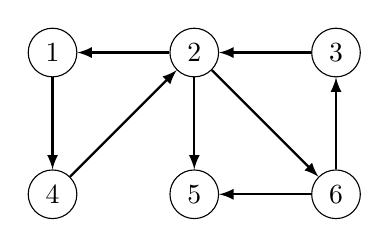
\begin{tikzpicture}[scale=0.9]
\node[draw, circle] (1) at (1,3) {$1$};
\node[draw, circle] (2) at (1,1) {$4$};
\node[draw, circle] (3) at (3,3) {$2$};
\node[draw, circle] (4) at (5,3) {$3$};
\node[draw, circle] (5) at (3,1) {$5$};
\node[draw, circle] (6) at (5,1) {$6$};

\path[draw,thick,->,>=latex] (1) -- (2);
\path[draw,thick,->,>=latex] (2) -- (3);
\path[draw,thick,->,>=latex] (3) -- (1);
\path[draw,thick,->,>=latex] (4) -- (3);
\path[draw,thick,->,>=latex] (3) -- (5);
\path[draw,thick,->,>=latex] (3) -- (6);
\path[draw,thick,->,>=latex] (6) -- (4);
\path[draw,thick,->,>=latex] (6) -- (5);
\end{tikzpicture}
\end{center}
其邻接矩阵为
\[
V= \begin{bmatrix}
  0 & 0 & 0 & 1 & 0 & 0 \\
  1 & 0 & 0 & 0 & 1 & 1 \\
  0 & 1 & 0 & 0 & 0 & 0 \\
  0 & 1 & 0 & 0 & 0 & 0 \\
  0 & 0 & 0 & 0 & 0 & 0 \\
  0 & 0 & 1 & 0 & 1 & 0 \\
 \end{bmatrix}.
\]
例如，矩阵
\[
V^4= \begin{bmatrix}
  0 & 0 & 1 & 1 & 1 & 0 \\
  2 & 0 & 0 & 0 & 2 & 2 \\
  0 & 2 & 0 & 0 & 0 & 0 \\
  0 & 2 & 0 & 0 & 0 & 0 \\
  0 & 0 & 0 & 0 & 0 & 0 \\
  0 & 0 & 1 & 1 & 1 & 0 \\
 \end{bmatrix}
\]
包含各结点对之间恰好有 4 条边的路径数量。例如，$V^4[2,5]=2$，因为从结点 2 到结点 5 恰好有两条包含 4 条边的路径：
$2 \rightarrow 1 \rightarrow 4 \rightarrow 2 \rightarrow 5$
以及
$2 \rightarrow 6 \rightarrow 3 \rightarrow 2 \rightarrow 5$.

\subsubsection{最短路}

在带权图中利用类似思想，可以计算每对结点之间恰好包含 $n$ 条边的最短路径长度。为此，需要重新定义矩阵乘法，使其不再统计路径数量，而是最小化路径长度。

\begin{samepage}
例如，考虑下图：
\begin{center}
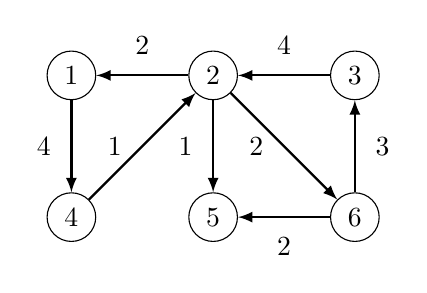
\begin{tikzpicture}[scale=0.9]
\node[draw, circle] (1) at (1,3) {$1$};
\node[draw, circle] (2) at (1,1) {$4$};
\node[draw, circle] (3) at (3,3) {$2$};
\node[draw, circle] (4) at (5,3) {$3$};
\node[draw, circle] (5) at (3,1) {$5$};
\node[draw, circle] (6) at (5,1) {$6$};

\path[draw,thick,->,>=latex] (1) -- node[font=\small,label=left:4] {} (2);
\path[draw,thick,->,>=latex] (2) -- node[font=\small,label=left:1] {} (3);
\path[draw,thick,->,>=latex] (3) -- node[font=\small,label=north:2] {} (1);
\path[draw,thick,->,>=latex] (4) -- node[font=\small,label=north:4] {} (3);
\path[draw,thick,->,>=latex] (3) -- node[font=\small,label=left:1] {} (5);
\path[draw,thick,->,>=latex] (3) -- node[font=\small,label=left:2] {} (6);
\path[draw,thick,->,>=latex] (6) -- node[font=\small,label=right:3] {} (4);
\path[draw,thick,->,>=latex] (6) -- node[font=\small,label=below:2] {} (5);
\end{tikzpicture}
\end{center}
\end{samepage}

构造一个邻接矩阵，其中 $\infty$ 表示不存在边，其他数值表示边权。矩阵为
\[
V= \begin{bmatrix}
  \infty & \infty & \infty & 4 & \infty & \infty \\
  2 & \infty & \infty & \infty & 1 & 2 \\
  \infty & 4 & \infty & \infty & \infty & \infty \\
  \infty & 1 & \infty & \infty & \infty & \infty \\
  \infty & \infty & \infty & \infty & \infty & \infty \\
  \infty & \infty & 3 & \infty & 2 & \infty \\
 \end{bmatrix}.
\]

不再使用公式
\[
AB[i,j] = \sum_{k=1}^n A[i,k] \cdot B[k,j]
\]
而使用公式
\[
AB[i,j] = \min_{k=1}^n A[i,k] + B[k,j]
\]
进行矩阵乘法。也就是说，以取最小值代替求和，以元素相加代替相乘。经过这一修改，矩阵幂就对应图中的最短路。

例如，由于
\[
V^4= \begin{bmatrix}
  \infty & \infty & 10 & 11 & 9 & \infty \\
  9 & \infty & \infty & \infty & 8 & 9 \\
  \infty & 11 & \infty & \infty & \infty & \infty \\
  \infty & 8 & \infty & \infty & \infty & \infty \\
  \infty & \infty & \infty & \infty & \infty & \infty \\
  \infty & \infty & 12 & 13 & 11 & \infty \\
 \end{bmatrix},
\]
可以得出：从结点 2 到结点 5、恰好包含 4 条边的路径最短长度为 8。这样的一条路径是 $2 \rightarrow 1 \rightarrow 4 \rightarrow 2 \rightarrow 5$。

\subsubsection{Kirchhoff 定理}

\index{Kirchhoff's theorem}
\index{spanning tree}

\key{Kirchhoff 定理}
%\footnote{G. R. Kirchhoff (1824--1887) was a German physicist.}
给出了一种方法，可以通过一个特殊矩阵的行列式计算图的生成树数量。例如，图
\begin{center}
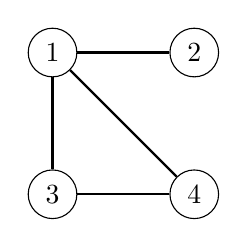
\begin{tikzpicture}[scale=0.9]
\node[draw, circle] (1) at (1,3) {$1$};
\node[draw, circle] (2) at (3,3) {$2$};
\node[draw, circle] (3) at (1,1) {$3$};
\node[draw, circle] (4) at (3,1) {$4$};

\path[draw,thick,-] (1) -- (2);
\path[draw,thick,-] (1) -- (3);
\path[draw,thick,-] (3) -- (4);
\path[draw,thick,-] (1) -- (4);
\end{tikzpicture}
\end{center}
有三棵生成树：
\begin{center}
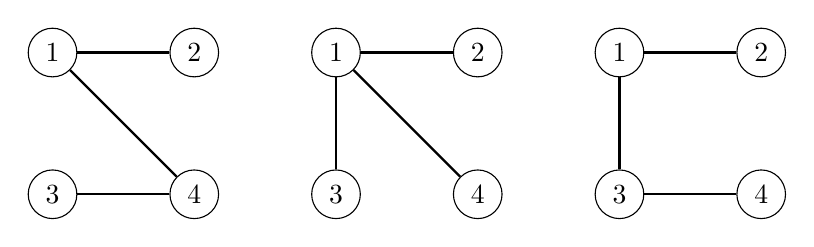
\begin{tikzpicture}[scale=0.9]
\node[draw, circle] (1a) at (1,3) {$1$};
\node[draw, circle] (2a) at (3,3) {$2$};
\node[draw, circle] (3a) at (1,1) {$3$};
\node[draw, circle] (4a) at (3,1) {$4$};

\path[draw,thick,-] (1a) -- (2a);
%\path[draw,thick,-] (1a) -- (3a);
\path[draw,thick,-] (3a) -- (4a);
\path[draw,thick,-] (1a) -- (4a);

\node[draw, circle] (1b) at (1+4,3) {$1$};
\node[draw, circle] (2b) at (3+4,3) {$2$};
\node[draw, circle] (3b) at (1+4,1) {$3$};
\node[draw, circle] (4b) at (3+4,1) {$4$};

\path[draw,thick,-] (1b) -- (2b);
\path[draw,thick,-] (1b) -- (3b);
%\path[draw,thick,-] (3b) -- (4b);
\path[draw,thick,-] (1b) -- (4b);

\node[draw, circle] (1c) at (1+8,3) {$1$};
\node[draw, circle] (2c) at (3+8,3) {$2$};
\node[draw, circle] (3c) at (1+8,1) {$3$};
\node[draw, circle] (4c) at (3+8,1) {$4$};

\path[draw,thick,-] (1c) -- (2c);
\path[draw,thick,-] (1c) -- (3c);
\path[draw,thick,-] (3c) -- (4c);
%\path[draw,thick,-] (1c) -- (4c);
\end{tikzpicture}
\end{center}
\index{Laplacean matrix}
为了计算生成树数量，构造\key{Laplacian 矩阵} $L$：$L[i,i]$ 为结点 $i$ 的度；若结点 $i$、$j$ 之间有边，则 $L[i,j]=-1$，否则 $L[i,j]=0$。上图的 Laplacian 矩阵为：
\[
L= \begin{bmatrix}
  3 & -1 & -1 & -1 \\
  -1 & 1 & 0 & 0 \\
  -1 & 0 & 2 & -1 \\
  -1 & 0 & -1 & 2 \\
 \end{bmatrix}
\]

可以证明，从 $L$ 中删除任意一行和任意一列所得矩阵的行列式，就等于生成树数量。例如，删除第一行和第一列后得到

\[ \det(
\begin{bmatrix}
  1 & 0 & 0 \\
  0 & 2 & -1 \\
  0 & -1 & 2 \\
 \end{bmatrix}
) =3.\]
无论从 $L$ 中删除哪一行、哪一列，所得行列式的值始终相同。

注意，第 22.5 节的 Cayley 公式是 Kirchhoff 定理的一个特例，因为对于含 $n$ 个结点的完全图，

\[ \det(
\begin{bmatrix}
  n-1 & -1 & \cdots & -1 \\
  -1 & n-1 & \cdots & -1 \\
  \vdots & \vdots & \ddots & \vdots \\
  -1 & -1 & \cdots & n-1 \\
 \end{bmatrix}
) =n^{n-2}.\]
